\section{Position-sensitive detector}

\subsection{Transverse photoeffect}

% TODO: cite Simon13

\begin{figure}[H]
	\centering
	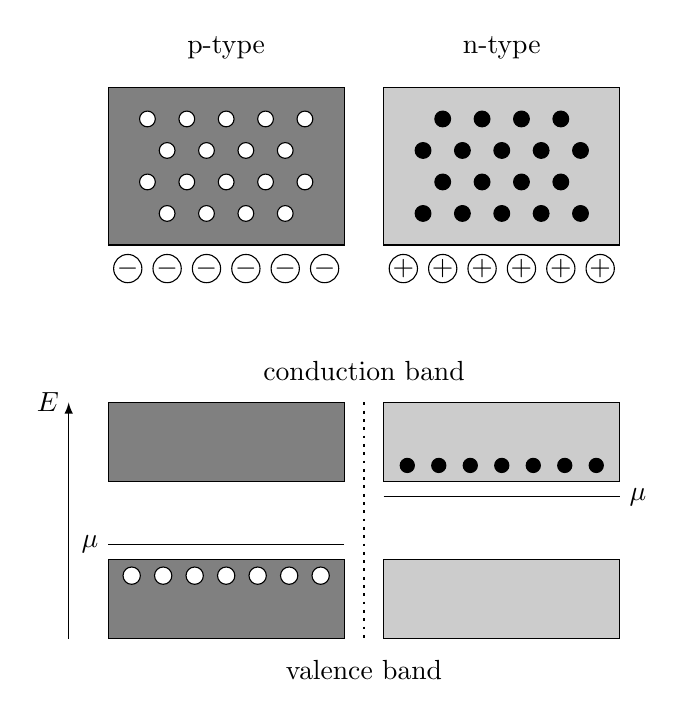
\begin{tikzpicture}
		\draw (1.5, 2.5) node {p-type};
		\draw (5, 2.5) node {n-type};
		\filldraw[draw=black, fill=gray] (0, 0) rectangle (3, 2);
		\filldraw[draw=black, fill=gray!40] (3.5, 0) rectangle (6.5, 2);
		\foreach \x in {1, ..., 4} {
			\filldraw[fill=white] (0.25+0.5*\x, 0.4) circle (.1);
			\filldraw[fill=white] (0.25+0.5*\x, 1.2) circle (.1);

			\filldraw[fill=black] (3.75+0.5*\x, 0.8) circle (.1);
			\filldraw[fill=black] (3.75+0.5*\x, 1.6) circle (.1);
		}
		\foreach \x in {1, ..., 5} {
			\filldraw[fill=white] (0.5*\x, 0.8) circle (.1);
			\filldraw[fill=white] (0.5*\x, 1.6) circle (.1);
			
			\filldraw[fill=black] (3.5+0.5*\x, 0.4) circle (.1);
			\filldraw[fill=black] (3.5+0.5*\x, 1.2) circle (.1);
		}
		\foreach \x in {0, ..., 5} {
			\draw (0.25+0.5*\x, -0.3) node[circle, draw=black, inner sep=0]{$-$};
			\draw (3.75+0.5*\x, -0.3) node[circle, draw=black, inner sep=0]{$+$};
		}
		\draw[-latex] (-0.5, -5) -- (-0.5, -2) node[left]{$E$};
		\draw[dotted, line width=1] (3.25, -2) -- (3.25, -5);
		\filldraw[draw=black, fill=gray] (0, -2) rectangle +(3, -1) +(0, -1.8) node[left]{$\mu$} -- +(3, -1.8) ++(0, -2) rectangle +(3, -1);
		\filldraw[draw=black, fill=gray!40] (3.5, -2) rectangle +(3, -1) +(0, -1.2) -- +(3, -1.2) node[right]{$\mu$} ++(0, -2) rectangle +(3, -1);
		\draw (3.25, -1.6) node{conduction band} +(0, -3.8) node{valence band};
		\foreach \x in {0, ..., 6} {
			\filldraw[fill=white] (0.3+0.4*\x, -4.2) circle (.11);
			\filldraw[fill=black] (3.8+0.4*\x, -2.8) circle (.09);
		}
	\end{tikzpicture}
	\caption{Separated p- and n-type semiconductor with holes (white) and electrons (black).}
\end{figure}

\begin{figure}[H]
	\centering
	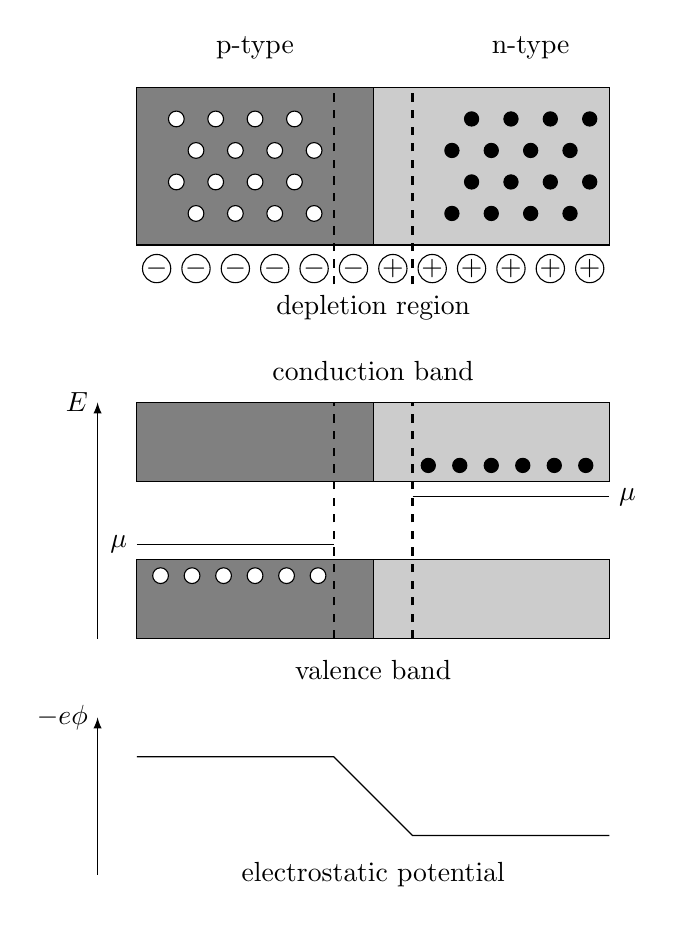
\begin{tikzpicture}
		\draw (1.5, 2.5) node {p-type};
		\draw (5, 2.5) node {n-type};
		\filldraw[draw=black, fill=gray] (0, 0) rectangle (3, 2);
		\filldraw[draw=black, fill=gray!40] (3, 0) rectangle (6, 2);
		\foreach \x in {1, ..., 4} {
			\filldraw[fill=white] (0.25+0.5*\x, 0.4) circle (.1);
			\filldraw[fill=white] (0.25+0.5*\x, 1.2) circle (.1);

			\filldraw[fill=black] (3.75+0.5*\x, 0.8) circle (.09);
			\filldraw[fill=black] (3.75+0.5*\x, 1.6) circle (.09);
		}
		\foreach \x in {1, ..., 4} {
			\filldraw[fill=white] (0.5*\x, 0.8) circle (.1);
			\filldraw[fill=white] (0.5*\x, 1.6) circle (.1);
			
			\filldraw[fill=black] (3.5+0.5*\x, 0.4) circle (.09);
			\filldraw[fill=black] (3.5+0.5*\x, 1.2) circle (.09);
		}
		\foreach \x in {0, ..., 5} {
			\draw (0.25+0.5*\x, -0.3) node[circle, draw=black, inner sep=0]{$-$};
			\draw (3.25+0.5*\x, -0.3) node[circle, draw=black, inner sep=0]{$+$};
		}
		\draw[dashed, line width=.8] (2.5, -.5) -- +(0, 2.5) +(1, 0) -- +(1, 2.5) +(0.5, -0.3) node{depletion region};

		\draw[-latex] (-0.5, -5) -- (-0.5, -2) node[left]{$E$};
		\filldraw[draw=black, fill=gray] (0, -2) rectangle +(3, -1) +(0, -1.8) node[left]{$\mu$} -- +(2.5, -1.8) ++(0, -2) rectangle +(3, -1);
		\filldraw[draw=black, fill=gray!40] (3, -2) rectangle +(3, -1) +(0.5, -1.2) -- +(3, -1.2) node[right]{$\mu$} ++(0, -2) rectangle +(3, -1);
		\draw[dashed, line width=.8] (2.5, -5) -- +(0, 3) +(1, 0) -- +(1, 3) +(0.5, -0.3);
		\draw (3, -1.6) node{conduction band} +(0, -3.8) node{valence band};
		\foreach \x in {0, ..., 5} {
			\filldraw[fill=white] (0.3+0.4*\x, -4.2) circle (.10);
			\filldraw[fill=black] (3.7+0.4*\x, -2.8) circle (.09);
		}
		
		\draw[-latex] (-0.5, -8) -- (-0.5, -6) node[left]{$-e\phi$};
		\draw (0, -6.5) -- ++(2.5, 0) -- ++(1, -1) -- ++(2.5, 0);
		\draw (3, -8) node{electrostatic potential};
	\end{tikzpicture}
	\caption{Junction, energy and electrostatic potential of p- and n-type semiconductor with holes (white) and electrons (black).}
\end{figure}

\begin{figure}[H]
	\centering
	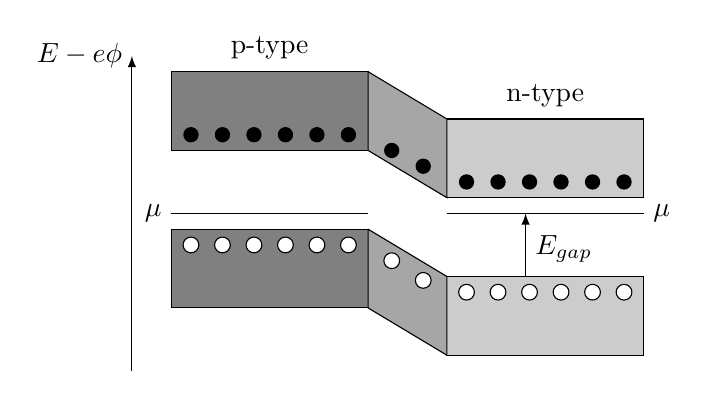
\begin{tikzpicture}
		\draw (1.25, 3.6) node {p-type};
		\draw (4.75, 3.0) node {n-type};
		\draw[-latex] (-0.5, -0.5) -- (-0.5, 3.5) node[left]{$E-e\phi$};
		\filldraw[draw=black, fill=gray] (0, 3.3) rectangle +(2.5, -1) +(0, -1.8) node[left]{$\mu$} -- +(2.5, -1.8) ++(0, -2) rectangle +(2.5, -1);
		\filldraw[draw=black, fill=gray!40] (3.5, 2.7) rectangle +(2.5, -1) +(0, -1.2) -- +(2.5, -1.2) node[right]{$\mu$} ++(0, -2) rectangle +(2.5, -1);
		\filldraw[draw=black, fill=gray!70] (2.5, 3.3) -- ++(1, -.6) -- ++(0, -1) -- ++(-1, .6) -- ++(0, 1);
		\filldraw[draw=black, fill=gray!70] (2.5, 1.3) -- ++(1, -.6) -- ++(0, -1) -- ++(-1, .6) -- ++(0, 1);
		\draw[-latex] (4.5, 0.7) -- ++(0, 0.8);
		\draw (4.5, 1.05) node[right]{$E_\text{gap}$};
		\foreach \x in {0, ..., 5} {
			\filldraw[fill=white] (0.25+0.4*\x, 1.1) circle (.10);
			\filldraw[fill=white] (3.75+0.4*\x, 0.5) circle (.10);
			\filldraw[fill=black] (3.75+0.4*\x, 1.9) circle (.09);
			\filldraw[fill=black] (0.25+0.4*\x, 2.5) circle (.09);
		};
		\filldraw[fill=white] (2.8, 0.9) circle (.10);
		\filldraw[fill=white] (3.2, 0.65) circle (.10);
		\filldraw[fill=black] (2.8, 2.3) circle (.09);
		\filldraw[fill=black] (3.2, 2.1) circle (.09);
	\end{tikzpicture}
	\caption{Energy of a p-n junction in equilibrium with holes (white) and electrons (black).}
\end{figure}

\begin{figure}[H]
	\centering
	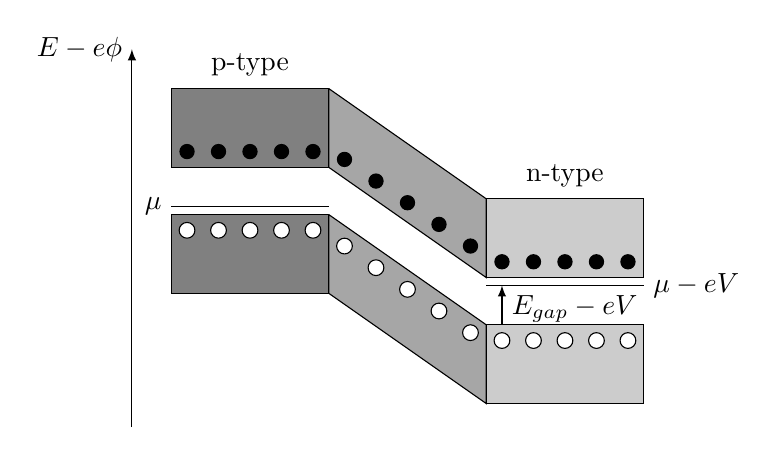
\begin{tikzpicture}
		\draw (1, 3.6) node {p-type};
		\draw (5, 2.2) node {n-type};
		\draw[-latex] (-0.5, -1) -- (-0.5, 3.8) node[left]{$E-e\phi$};
		\filldraw[draw=black, fill=gray] (0, 3.3) rectangle +(2, -1) +(0, -1.5) node[left]{$\mu$} -- +(2, -1.5) ++(0, -1.6) rectangle +(2, -1);
		\filldraw[draw=black, fill=gray!40] (4, 1.9) rectangle +(2, -1) +(0, -1.1) -- +(2, -1.1) node[right]{$\mu-eV$} ++(0, -1.6) rectangle +(2, -1);
		\filldraw[draw=black, fill=gray!70] (2, 3.3) -- ++(2, -1.4) -- ++(0, -1) -- ++(-2, 1.4) -- ++(0, 1);
		\filldraw[draw=black, fill=gray!70] (2, 1.7) -- ++(2, -1.4) -- ++(0, -1) -- ++(-2, 1.4) -- ++(0, 1);
		\draw[-latex] (4.2, 0.3) -- ++(0, 0.5);
		\draw (4.2, 0.5) node[right]{$E_\text{gap}-eV$};
		\foreach \x in {0, ..., 4} {
			\filldraw[fill=white] (0.2+0.4*\x, 1.5) circle (.10);
			\filldraw[fill=white] (2.2+0.4*\x, 1.3-0.275*\x) circle (.10);
			\filldraw[fill=white] (4.2+0.4*\x, 0.1) circle (.10);
			\filldraw[fill=black] (4.2+0.4*\x, 1.1) circle (.09);
			\filldraw[fill=black] (2.2+0.4*\x, 2.4-0.275*\x) circle (.09);
			\filldraw[fill=black] (0.2+0.4*\x, 2.5) circle (.09);
		};
	\end{tikzpicture}
	\caption{Energy diagram of a reverse biased p-n junction with holes (white) and electrons (black).}
\end{figure}

\begin{figure}[H]
	\centering
	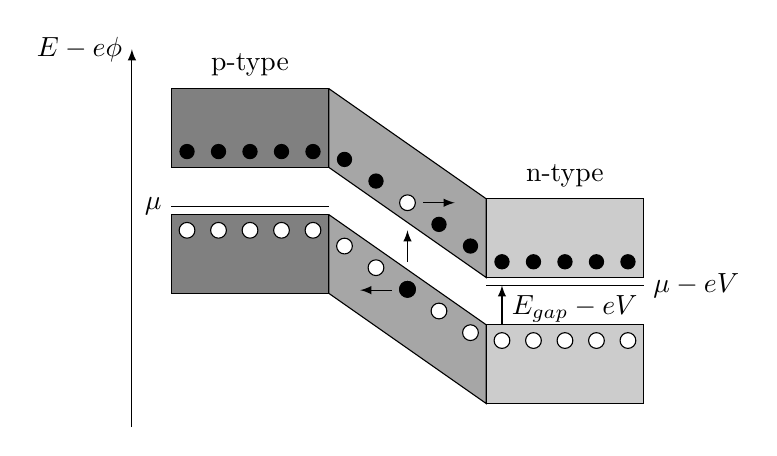
\begin{tikzpicture}
		\draw (1, 3.6) node {p-type};
		\draw (5, 2.2) node {n-type};
		\draw[-latex] (-0.5, -1) -- (-0.5, 3.8) node[left]{$E-e\phi$};
		\filldraw[draw=black, fill=gray] (0, 3.3) rectangle +(2, -1) +(0, -1.5) node[left]{$\mu$} -- +(2, -1.5) ++(0, -1.6) rectangle +(2, -1);
		\filldraw[draw=black, fill=gray!40] (4, 1.9) rectangle +(2, -1) +(0, -1.1) -- +(2, -1.1) node[right]{$\mu-eV$} ++(0, -1.6) rectangle +(2, -1);
		\filldraw[draw=black, fill=gray!70] (2, 3.3) -- ++(2, -1.4) -- ++(0, -1) -- ++(-2, 1.4) -- ++(0, 1);
		\filldraw[draw=black, fill=gray!70] (2, 1.7) -- ++(2, -1.4) -- ++(0, -1) -- ++(-2, 1.4) -- ++(0, 1);
		\draw[-latex] (4.2, 0.3) -- ++(0, 0.5);
		\draw (4.2, 0.5) node[right]{$E_\text{gap}-eV$};
		\foreach \x in {0, ..., 4} {
			\filldraw[fill=white] (0.2+0.4*\x, 1.5) circle (.10);
			\filldraw[fill=white] (2.2+0.4*\x, 1.3-0.275*\x) circle (.10);
			\filldraw[fill=white] (4.2+0.4*\x, 0.1) circle (.10);
			\filldraw[fill=black] (4.2+0.4*\x, 1.1) circle (.09);
			\filldraw[fill=black] (2.2+0.4*\x, 2.4-0.275*\x) circle (.09);
			\filldraw[fill=black] (0.2+0.4*\x, 2.5) circle (.09);
		};
		\filldraw[fill=white] (3.0, 1.85) circle (.10);
		\filldraw[fill=black] (3.0, 0.75) circle (.10);
		\draw[-latex] (3.0, 1.1) -- +(0, 0.4);
		\draw[-latex] (3.2, 1.85) -- +(0.4, 0);
		\draw[-latex] (2.8, 0.74) -- +(-0.4, 0);
	\end{tikzpicture}
	\caption{Energy diagram of a reverse biased p-n junction under illumination with holes (white) and electrons (black).}
\end{figure}

\begin{equation}
	I_\text{dark}=I_\text{sat}\left(e^{e_0V_d/k_BT}-1\right)
\end{equation}

\subsection{Lateral photoeffect}

% TODO: lateral photoeffect Schottky30, Wallmark57

The lateral photoeffect was first discovered by W. Schottky in 1930~\cite{Schottky30}.
In 1957, it was rediscovered by J. Wallmark~\cite{Wallmark57}.

% TODO: Lucovsky equations Woltring paper
% TODO: pin-cushion type Doke87, Wang89
% TODO: overview of position-sensitive detectors and why we choose the lateral pin-cushion type
% TODO: diagram of depletion region for lateral photodiode


% TODO: photodiode characteristics
% TODO: diode leakage current
% TODO: responsitivity
% TODO: bandwidth limit
% TODO: motivate value for reverse bias

% TODO: noise model
% TODO: photon shot noise

\begin{figure}[H]
	\centering
	\begin{circuitikz}
		\draw (0, 0) node[circ]{};
		\draw (+2, +2) node[ocirc, label=X1]{} to[photodiode] (0, 0);
		\draw (-2, -2) node[ocirc, label=X2]{} to[photodiode] (0, 0);
		\draw (+2, -2) node[ocirc, label=Y2]{} to[photodiode] (0, 0);
		\draw (-2, +2) node[ocirc, label=Y1]{} to[photodiode] (0, 0);
		\draw (0, 0) -- ++(0, -2.5) node[ocirc, label=Cathode, rotate=180]{};
	\end{circuitikz}
	\caption{Position-sensitive detector as photodiodes}
\end{figure}

% TODO: mention non-linearity of voltage response to illumination

\begin{figure}[H]
	% TODO: add position dependent potentiometers to anode (Andersson08 Fig. 15) 
	\centering
	\begin{circuitikz}
		\draw (-3, -2) to[current source, l=$I_\text{photo}$] ++(0, 4);
		\draw (-1, -2) node[circ]{} to[current source, l=$I_\text{dark}$] ++(0, 4) node[circ]{};
		\draw (1, -2) node[circ]{} to[resistor, l=$R_d$] ++(0, 4) node[circ]{};
		\draw (3, -2) to[capacitor, l=$C_d$] ++(0, 4);
		\draw (-3, -2) -- ++(6, 0);
		\draw (-3, 2) -- ++(6, 0);
		\draw (0, -2) -- ++(0, -1) node[ocirc, label=Cathode, rotate=180]{};
		\draw (0, 2) -- ++(0, 1) node[ocirc, label=Anode]{};
	\end{circuitikz}
	\caption{Photodiode equivalent circuit}
\end{figure}